\chapter{Raspberry PI}\label{cap:revisao}

Nesse capítulo serão apresentadas as ferramentas utilizados na implementação do projeto...

\section{Raspberry Pi 3 Versão B}

%% Falar das caracteristicas do hardware e sua comfiguração

\subsection{Motivação do uso do Raspberry}

%%Deixa essa comigo

\subsection{Métodos de instalação do Raspbian}

%%Falar sobre o noobs e a instalação direta em um passo-a-passo.

\subsection{Bitcoin Core}

%%Descrever os passos de compilação e instalação e mencionar a existencia do repositório apt-get no fim

O tipo de estudo mencionado acima, na QS2, provém da classificação apresentada
em \cite{wieringa2006requirements} e é descrita brevemente abaixo. Essas classes
foram usadas também em \cite{Kuhrmann:2015:SPI:2785592.2785600}.
  


Com essas indagações, pudemos construir e ajustar \textit{strings} de buscas de
forma que resultassem em possíveis respostas , até que chegássemos em uma
\textit{string} definitiva.


\begin{itemize}
\setlength{\itemsep}{1pt}
\setlength{\itemindent}{20pt}
\item {(("\textit{software}") AND ("\textit{scope}" OR
"\textit{requirements}") AND ("\textit{negotiation}"))}
\end{itemize}

A população (\textit{population}) da \textit{String} acima é definida por
'\textit{software}', '\textit{scope}' e '\textit{requirements}'; a intervenção (\textit{Intervention}) é definida como
'\textit{negotiation}'.
Não há na \textit{string} comparação (Comparison), já que não restringimos
nossos resultados aos artigos que comparem técnicas, como não há também uma definição
de resultados (Outcome), a fim de não haver nenhum tipo de restrição.

As próximas etapas deverão ser realizadas considerando os critérios de inclusão
e de exclusão. Definimos que se os pesquisadores discordarem sobre a
conformidade do artigo com esses critérios, um terceiro pesquisador faria também
uma avaliação. Esses critérios de inclusão e de exclusão são apresentados a
seguir.

Inclusão:
\begin{itemize}
\setlength{\itemsep}{1pt}
\setlength{\itemindent}{20pt}
\item {Artigos que descrevem, propõem, aplicam ou avaliam técnicas de negociação
de requisitos.}
\end{itemize}

Exclusão:
\begin{itemize}
\setlength{\itemsep}{1pt}
\setlength{\itemindent}{20pt}
\item {Artigos que não descrevem os passos de uma técnica de maneira
compreensível.}
\item {Artigos onde a técnica é somente mencionada.}
\item {Artigos em outros idiomas que não o inglês, para facilitar a reprodução
do protocolo em qualquer lugar do mundo.}
\item {Artigos que descrevem técnicas de negociação para contextos não presenciais (\textit{e.g.}, distribuídas).}
\end{itemize}

Para mensurar a eficiência de nossa \textit{String}, estipulamos alguns artigos
relevantes e que atendem as exigências impostas pelos critérios de inclusão,
exclusão e a definição do tema de pesquisa. Estes, chamados artigos de controle,
deveriam ser retornados como resultados da busca na biblioteca digital escolhida
e se encontram adiante.

\begin{enumerate}
\setlength{\itemsep}{1pt}
\setlength{\itemindent}{20pt}
\item \textit{software requirements negotiation using the software quality
function deployment \cite{ramires2005software}
  \item Integration of scrum with Win-Win requirements negotiation
  model \cite{khan2014integration}
\item Requirements Negotiation Using Multi-Criteria Preference
Analysis \cite{in2004requirements}}
\end{enumerate}

Os artigos resultantes da busca na biblioteca Scopus, seriam então analisados
por título e \textit{abstract}, levando em consideração o tema da pesquisa, os
critérios de inclusão e os critérios de exclusão.
Essa análise, naturalmente resultaria em dois conjuntos, o conjunto de artigos
aprovados e o conjunto de artigos reprovados. O primeiro destes, seria o ponto
de partida para a próxima etapa de filtragem, a filtragem por conteúdo.
Essa etapa consiste em os pesquisadores lerem cada artigo e avaliarem, segundo
os mesmos critérios já apresentados, se os artigos são ou não pertinentes para atingir o objetivo da pesquisa.
 Os artigos pertinentes serviriam como conjunto para a aplicação da técnica
 \textit{snowballing}, que contribui para a garantia da eficiência em encontrar
 artigos relevantes, sem perda de completude, quando comparada com buscar com a
 mesma \textit{String} em diferentes bibliotecas digitais
 \cite{Badampudi:2015:EUS:2745802.2745818}.
 
Com os artigos encontrados ao se aplicar o \textit{snowballing}, realizar-se-ia
a primeira e a segunda filtragem.
Este processo de filtragem e \textit{snowballing} é iterativo e possui como
condição de parada a não obtenção de novos resultados.

Com o conjunto final de todos os artigos, extrair-se-ão os dados a seguir.

\begin{itemize}
\setlength{
\itemsep}{1pt}
\setlength{
\itemindent}{20pt}
\item {Referência.}
\item {Nome da técnica.}
\item {Tem negociação de requisitos como alvo principal?}
\item {Descrição resumida da técnica (ou da parte referente à negociação de requisitos).}
\item {Ambiente (academia ou indústria).}
\item {Tipo de pesquisa (\textit{Evaluation research,
Solution proposal, Philosophical paper, Opinion paper, Experience paper)}.}
\item {Tipo de estudo primário (experimento, estudo de caso ou
\textit{survey}).}
\item {Achados principais do artigo (conhecimento gerado).}
\item {Vantagens.}
\item {Desvantagens.}
\end{itemize}

\section{Execução}

A \textit{string} de busca precisou ser adaptada para o formato da biblioteca
Scopus e o resultado dessa adaptação encontra-se a seguir.
 
 \begin{itemize}
\setlength{\itemsep}{1pt}
\setlength{\itemindent}{20pt}
\item {(("\textit{software}") AND ("\textit{scope}" OR "\textit{requirements}") AND ("negotiation" ))
AND ( LIMIT-TO(SUBJAREA,"COMP" ) OR LIMIT-TO(SUBJAREA,"ENGI" ) )}
\end{itemize}
 
A busca na biblioteca foi feita em 24 de novembro de 2015 e resultou em 408
artigos, que podem ser encontrados no apêndice. Esses, foram lidos e
filtrados como descrito no planejamento.
O conjunto obtido após a primeira filtragem continha 39 artigos e, após
a segunda filtragem restaram 18, que estão indicados no apêndice pela
cor cinza.

O segundo dos artigos de controle`, \cite{khan2014integration}, não havia sido
capturado devido a restrição por área (computação e engenharia), que foi posta,
a fim de que resultados de administração e economia, por exemplo, não fossem retornados. O motivo
para o artigo de controle não ter sido um dos resultados foi que o mesmo havia
sido cadastrado como 'multiarea'. A forma que foi indexado não é de nossa
compreensão, contudo entendemos que foi uma falha, visto que o mesmo é
claramente da área de computação. Este, então, também teve seus dados extraídos
e está contido nos 18 artigos mencionados.

 A busca na base Scopus permitiu obter de forma imparcial um conjunto de artigos que pudesse ser utilizado
 como \textit{seed set} para dar início ao \textit{backward snowballing}, que
 consiste em capturar todas as referências encontradas para cada um dos artigos
 do \textit{seed set}. O número total de referências foi de 383. Realizamos
 então a filtragem por título e, sendo assim, restaram 96, que continham
 duplicadas e removendo-as restaram 56. A filtragem por abstract reduziu o número à 26, entretanto desses somente 21 foram encontrados para filtragem por conteúdo e, esta última filtragem resultou em 15 artigos válidos,
que tiveram suas informações extraídas.

A Figura 2.1 representa como os artigos do
\textit{seed set} se relacionam em termos de citeções, enquanto a figura 2.2
mostra como todos os artigos encontrados estão relacionados em termos de
citações, sejam eles do \textit{seed set} ou provenientes do \textit{backward
snowballing}.

\begin{figure}[ht]
 \centering
 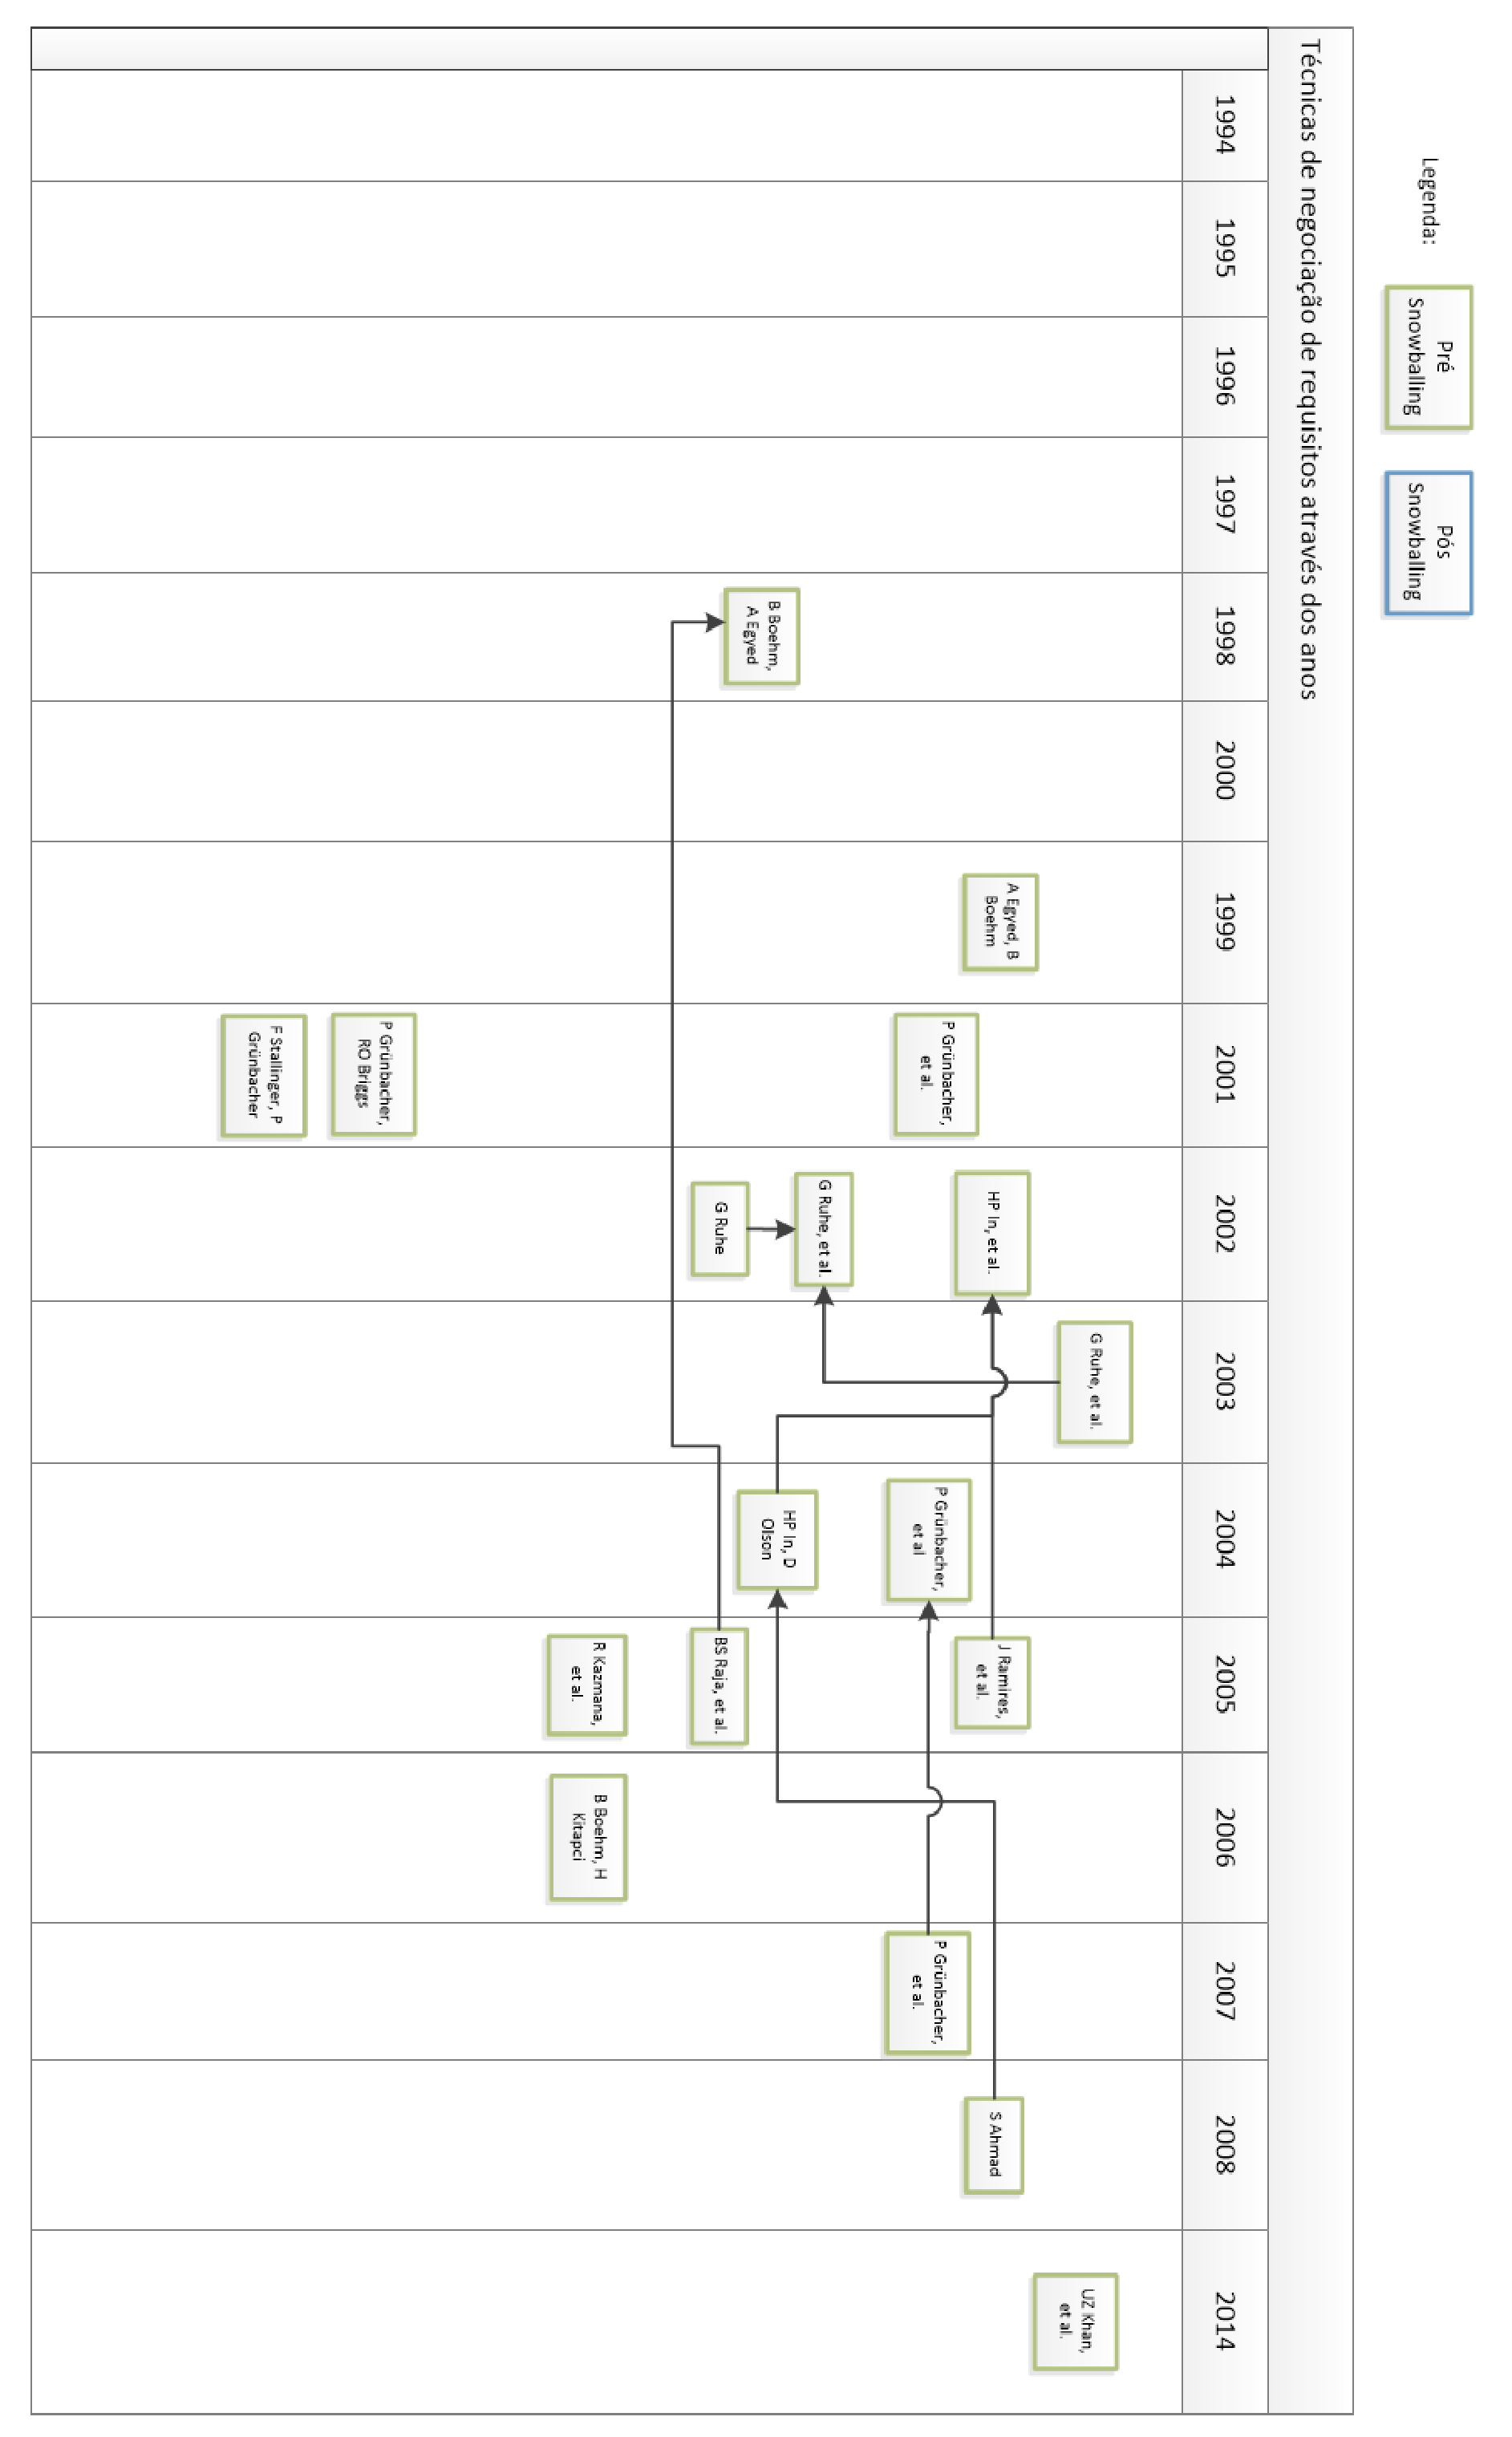
\includegraphics[scale=0.47]{pre_sb.eps}
 \caption{\label{fig:presb}Diagrama de Citações Pré \textit{Backward
 Snowballing}}
\end{figure}

\FloatBarrier

\begin{figure}[ht]
 \centering
 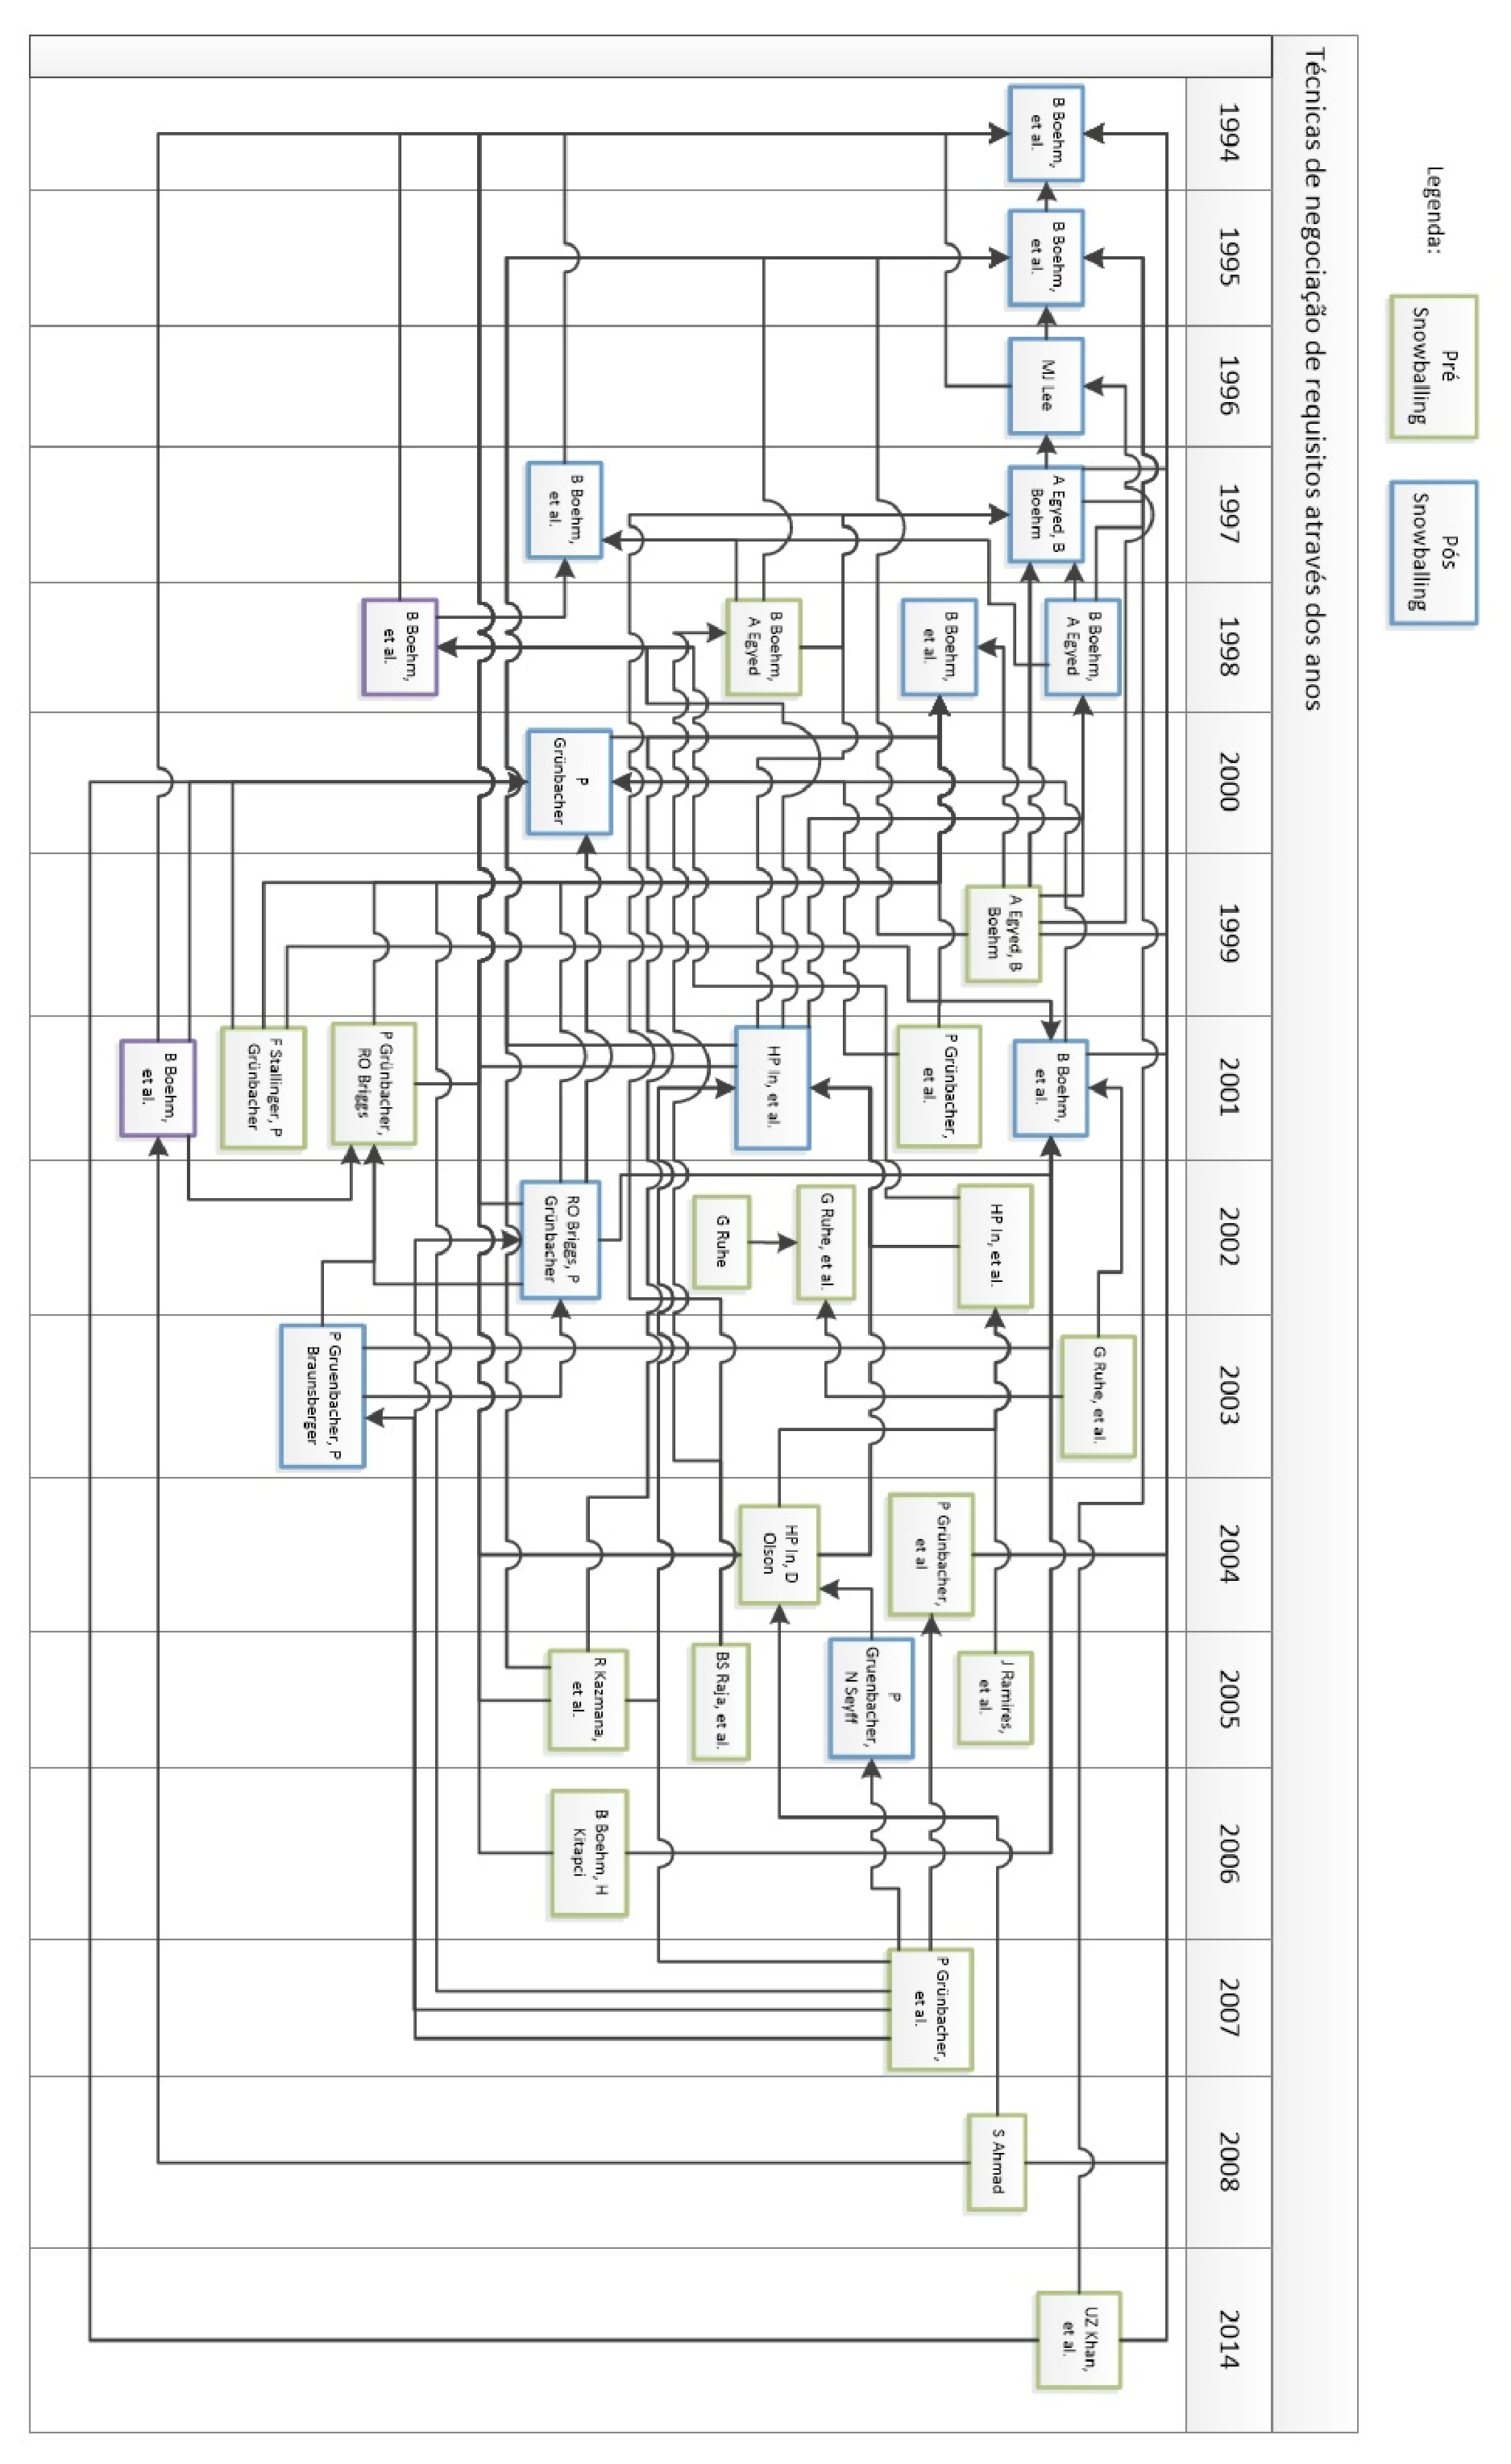
\includegraphics[scale=0.48]{final_sb.eps}
 \caption{\label{fig:possb}Diagrama de Citações pós \textit{Backward
 Snowballing}}
\end{figure}

\FloatBarrier

\section{Dados Extraídos}

Esta seção tem como objetivo apresentar os dados extraídos para cada um dos 33
artigos encontrados após a execução do protocolo da revisão quasi-sistemática.
Esses dados foram agrupados e debatidos para que pudéssemos responder as
questões de pesquisa, que foram apresentadas na seção do planejamento deste capítulo.
Essas respostas serão apresentadas no capítulo 3.


\begin{longtable}{{|>{\centering\arraybackslash}m{3cm}|>{\centering\arraybackslash}m{10cm}|}}
\caption{\label{fig:t1}Comparing software system requirements negotiation
patterns. Systems Engineering}\\
\hline 
\textbf{Referência}                                         & EGYED, Alexander;
BOEHM, Barry. \textit{Comparing software system requirements negotiation
patterns.}
\textit{Systems Engineering}, v. 2, n. 1, p. 1-14, 1999.
\cite{egyed1999comparing} \\ \hline \textbf{Nome da técnica}                                    & \textit{WinWIn}                    \\
\hline
\textbf{O foco é a negociação de requisitos?}               & Sim                       \\
\hline
\textbf{Descrição da técnica}                               & I                        \\
\hline
\textbf{Ambiente}                                           & Academia/indústria         \\
\hline
\textbf{Tipo de pesquisa}                                   & \textit{Evaluation
research}        \\
\hline
\textbf{Tipo de estudo primário (quando houver)}            & estudo de caso             \\
\hline
\textbf{Achados Principais do Artigo (Conhecimento Gerado)} & Foi verificado que clientes e usuários são mais presentes na etapa de identificação das condições de vitória, enquanto os desenvolvedores foram mais presentes na definição de problemas e nas suas opções de resolução. \\ \hline
\textbf{Vantagens}                                          &                          \\
\hline
\textbf{Desvantagens}                                       &                          \\
\hline

\end{longtable}

\begin{longtable}{{|>{\centering\arraybackslash}m{3cm}|>{\centering\arraybackslash}m{10cm}|}}
\caption{\label{fig:t2}Making every student a winner: The WinWin approach in
software engineering education.}\\
\hline 
\textbf{Referência}                                         & GRÜNBACHER, Paul
et al. Making every student a winner: The WinWin approach in software
engineering education. Journal of Systems and software, v. 80, n. 8, p.
1191-1200, 2007. \cite{grunbacher2007making} \\ \hline \textbf{Nome da técnica}                          
& \textit{WinWIn}                                                                                                                                                                          \\ \hline \textbf{O foco é a negociação de requisitos?}               & Sim                                                                                                                                                                             \\ \hline \textbf{Descrição da técnica}                               & I                                                                                                                                                                               \\ \hline \textbf{Ambiente}                                           & Academia                                                                                                                                                                        \\ \hline
\textbf{Tipo de pesquisa}                                   & \textit{Solution proposal}                                                                                                                                                                \\ \hline
\textbf{Tipo de estudo primário (quando houver)}            & Estudo de caso                                                                                                                                                              \\ \hline
\textbf{Achados Principais do Artigo (Conhecimento Gerado)} & Os alunos se sentem mais motivados a participar quando existe um papel de facilitador.                                                                                          \\ \hline
\textbf{Vantagens}                                          & Estimula a comunicação, ajuda na reconciliação de pontos conflitantes, ajuda na identificação de problemas e incertezas, tal como na percepção de possíveis acordos.            \\ \hline
\textbf{Desvantagens}                                       & Foi mencionado em quase todos os relatos que era preciso mais tempo para ensinar a metodologia.                                                                                 \\ \hline

\end{longtable}


\begin{longtable}{{|>{\centering\arraybackslash}m{3cm}|>{\centering\arraybackslash}m{10cm}|}}
\caption{\label{fig:t3}Quantitative WinWin: a new method for decision support in
requirements negotiation}\\
\hline
\textbf{Referência}                                         & RUHE, Günther;
EBERLEIN, Armin; PFAHL, Dietmar. Quantitative WinWin: a new method for decision
support in requirements negotiation. In: Proceedings of the 14th international
conference on software engineering and knowledge engineering. ACM, 2002. p.
159-166. \cite{ruhe2002quantitative}                                            
\\ \hline \textbf{Nome da técnica}                                    &
\textit{Quantitative WinWin}                                                    
\\ \hline \textbf{O foco é a negociação de requisitos?}               & Sim                                                                                                                                                                                                                                                                                                                   \\ \hline \textbf{Descrição da técnica}                               & II                                                                                                                                                                                                                                                                                                                     \\ \hline \textbf{Ambiente}                                           & Academia                                                                                                                                                                                                                                                                                                              \\ \hline \textbf{Tipo de pesquisa}                                   & \textit{Solution proposal}                                                                                                                                                                                                                                                                                                     \\ \hline \textbf{Tipo de estudo primário (quando houver)}            & Estudo de caso                                                                                                                                                                                                                                                                                                        \\ \hline \textbf{Achados Principais do Artigo (Conhecimento Gerado)} &                                                                                                                                                                                                                                                                                                                       \\ \hline
\textbf{Vantagens}                                          & A técnica não se
baseia em questões subjetivas para sua tomada de decisão como se faz na
\textit{WinWin}. Muito pelo contrário, ela se utiliza de dados quantitativos para basear melhor sua tomada de decisão.                                                                                                                \\ \hline \textbf{Desvantagens}                                       & Foi feita apenas uma simulação utilizando dados da indústria, logo não há confirmação real de que a técnica funcionaria corretamente em situações maiores e mais complexas. Ela também necessita de uma estimativa bastante efetiva e precisa do esforço atrelado a cada requisito para que sua análise seja efetiva. \\ \hline

\end{longtable}



\begin{longtable}{{|>{\centering\arraybackslash}m{3cm}|>{\centering\arraybackslash}m{10cm}|}}
\caption{\label{fig:t4}Requirements Negotiation Using Multi-Criteria Preference Analysis}\\
\hline
\textbf{Referência}                                         & IN, Hoh Peter;
OLSON, David. Requirements Negotiation Using Multi-Criteria Preference Analysis.
J. UCS, v. 10, n. 4, p. 306-325, 2004. \cite{in2004requirements}                                      
\\ \hline \textbf{Nome da técnica}                                    & MPARN                                                                                                                                                                                                  \\ \hline \textbf{O foco é a negociação de requisitos?}               & Sim                                                                                                                                                                                                    \\ \hline \textbf{Descrição da técnica}                               & III                 
\\ \hline \textbf{Ambiente}                                           & Academia                                                                                                                                                                                               \\ \hline
\textbf{Tipo de pesquisa}                                   & \textit{Solution proposal}                                                                                                                                                                                      \\ \hline
\textbf{Tipo de estudo primário (quando houver)}            & Estudo de caso                                                                                                                                                                                         \\ \hline
\textbf{Achados Principais do Artigo (Conhecimento Gerado)} &                                                                                                                                                                                                        \\ \hline
\textbf{Vantagens}                                          & Análise de opções menos subjetiva e mais objetiva.                                                                                                                                                     \\ \hline
\textbf{Desvantagens}                                       & Não possui boa
solução para sistema de como se tomar a decisão final. Não foi feito nenhum experimento concreto sobre a eficácia da técnica, estudo de caso detalhado no artigo era hipotético. \\ \hline

\end{longtable}


\begin{longtable}{{|>{\centering\arraybackslash}m{3cm}|>{\centering\arraybackslash}m{10cm}|}}
\caption{\label{fig:t5}Multi-criteria preference analysis for systematic
requirements negotiation}\\
\hline
\textbf{Referência}                                         & IN, Hoh Peter;
OLSON, David; RODGERS, Tom. Multi-criteria preference analysis for systematic
requirements negotiation. In: Computer software and Applications Conference,
2002. COMPSAC 2002. Proceedings. 26th Annual International. IEEE, 2002. p.
887-892.  \cite{in2002multi}                                                                 
\\ \hline \textbf{Nome da técnica}                                    & MPARN                                                                                                                                                                                                                                                                                                                                                                                                                                                                                                                                                                                        \\ \hline \textbf{O foco é a negociação de requisitos?}               & Sim                                                                                                                                                                                                                                                                                                                                                                                                                                                                                                                                                                                          \\ \hline \textbf{Descrição da técnica}                               & III \\ \hline \textbf{Ambiente}                                           & Academia                                                                                                                                                                                                                                                                                                                                                                                                                                                                                                                                                                                     \\ \hline \textbf{Tipo de pesquisa}                                   & \textit{Solution proposal}                                                                                                                                                                                                                                                                                                                                                                                                                                                                                                                                                                          \\ \hline
\textbf{Tipo de estudo primário (quando houver)}            & estudo de caso                                                                                                                                                                                                                                                                                                                                                                                                                                                                                                                                                                               \\ \hline
\textbf{Achados Principais do Artigo (Conhecimento Gerado)} & Existem algumas
maneiras de guiar alguns dos passos apresentados no MPARN, por exemplo: No passo
5 pode-se usar um método direto, método com função linear, método com função não linear, método com progressão geométrica, existem,outros métodos não abordados no artigo. No passo 6: pode se usar um método subjetivo direto, método smart, método de comparação de razão em pares, método com progressão geométrica,ou outro que não foi dito no artigo. No passo 7: pode se usar forma democrática, democrática por meios aritméticos, democrática por meios geométricos ou ditatorial. \\ \hline \textbf{Vantagens}                                          &                                                                                                                                                                                                                                                                                                                                                                                                                                                                                                                                                                                              \\ \hline \textbf{Desvantagens}                                                                                                                                                                       &                                                                                                                                                                                                                                                               \\ \hline

\end{longtable}
\begin{longtable}{{|>{\centering\arraybackslash}m{3cm}|>{\centering\arraybackslash}m{10cm}|}}
\caption{\label{fig:t6}From requirements negotiation to software architecture
decisions}\\
\hline
\textbf{Referência}                                         & KAZMAN, Rick; IN,
Hoh Peter; CHEN, Hong-Mei. From requirements negotiation to software
architecture decisions. Information and software Technology, v. 47, n. 8, p.
511-520, 2005.  \cite{kazman2005requirements}                                                            
\\ \hline \textbf{Nome da técnica}                                    & Win CBAM                                                                                                                                                                                                                                                                                                                                                                                                                                   \\ \hline \textbf{O foco é a negociação de requisitos?}               & Sim                                                                                                                                                                                                                                                                                                                                                                                                                                        \\ \hline \textbf{Descrição da técnica}                               & IV \\ \hline \textbf{Ambiente}                                           & Academia/indústria                                                                                                                                                                                                                                                                                                                                                                                                                         \\ \hline
\textbf{Tipo de pesquisa}                                   & \textit{Evaluation research}                                                                                                                                                                                                                                                                                                                                                                                                                        \\ \hline
\textbf{Tipo de estudo primário (quando houver)}            & Estudo de caso                                                                                                                                                                                                                                                                                                                                                                                                                             \\ \hline
\textbf{Achados Principais do Artigo (Conhecimento Gerado)} &                                                                                                                                                                                                                                                                                                                                                                                                                                            \\ \hline
\textbf{Vantagens}                                          & A técnica captura
erro da quantificação pelos \textit{stakeholders} na etapa 5. A técnica agrega
valor não só na negociação de atributos de qualidade e de estratégias de arquitetura, mas
também consegue fornecer uma forma dos \textit{stakeholders} perceberem a ligação das
estratégias de arquitetura e dos atributos de qualidade com os requisitos,
possibilitando que os \textit{stakeholders} possam repensar os requisitos sob uma nova
perspectiva. \\ \hline \textbf{Desvantagens}                                    
& A técnica não apresenta forma de calcular o custo, pois supõe que a empresa já
adote alguma metodologia para isso                                                                                                                                                                                                                                                                                                                          \\ \hline
\end{longtable}



\begin{longtable}{{|>{\centering\arraybackslash}m{3cm}|>{\centering\arraybackslash}m{10cm}|}}
\caption{\label{fig:t7}The WinWin approach: using a requirements negotiation tool for rationale capture and use}\\
\hline
\textbf{Referência}                                         & BOEHM, Barry;
KITAPCI, Hasan. The WinWin approach: using a requirements negotiation tool for
rationale capture and use. In: Rationale management in software engineering.
Springer Berlin Heidelberg, 2006. p. 173-190. \cite{boehm2006winwin}                              
\\ \hline \textbf{Nome da técnica}                                    & \textit{WinWIn}                                                                                                                                                                                                                                                           \\ \hline \textbf{O foco é a negociação de requisitos?}               & Sim                                                                                                                                                                                                                                                              \\ \hline \textbf{Descrição da técnica}                               & I                                                                                                                                                                                                                                                                \\ \hline \textbf{Ambiente}                                           & Academia/indústria                                                                                                                                                                                                                                               \\ \hline
\textbf{Tipo de pesquisa}                                   & \textit{Experience paper}                                                                                                                                                                                                                                                 \\ \hline
\textbf{Tipo de estudo primário (quando houver)}            & Experimento                                                                                                                                                                                                                                                      \\ \hline
\textbf{Achados Principais do Artigo (Conhecimento Gerado)} & A equipe que usou o \textit{WinWIn} foi capaz de gerar resultados mais amplos e profundos. O \textit{WinWIn} também serve como forma de se documentar a tomada de decisão na negociação de requisitos.                                                                             \\ \hline
\textbf{Vantagens}                                          & A ferramenta EasyWinWin facilita a transição entre negociação de requisitos e especificação de requisitos.                                                                                                                                                       \\ \hline
\textbf{Desvantagens}                                       & A especificação de
requisitos gerada após o \textit{WinWIn}, tipicamente não é completa, precisa,
consistente e testável, pois vários dos requisitos podem ter sido permitidos durante a empolgação dos \textit{stakeholders} com o alto nível de cooperação durante a negociação. \\ \hline

\end{longtable}


\begin{longtable}{{|>{\centering\arraybackslash}m{3cm}|>{\centering\arraybackslash}m{10cm}|}}
\caption{\label{fig:t8}Trade-off analysis for requirements selection}\\
\hline
\textbf{Referência}                                         & RUHE, Günther;
EBERLEIN, Armin; PFAHL, Dietmar. Trade-off analysis for requirements selection.
International Journal of software Engineering and Knowledge Engineering, v. 13,
n. 04, p. 345-366, 2003. \cite{ruhe2003trade}                                                   
\\ \hline \textbf{Nome da técnica}                                    & \textit{Quantitative WinWin}                                                                                                                                                                                                                                                                                                   \\ \hline \textbf{O foco é a negociação de requisitos?}               & Sim                                                                                                                                                                                                                                                                                                                   \\ \hline \textbf{Descrição da técnica}                               & II                                                                                                                                                                                                                                                                                                                     \\ \hline \textbf{Ambiente}                                           & Academia                                                                                                                                                                                                                                                                                                              \\ \hline
\textbf{Tipo de pesquisa}                                   & \textit{Solution proposal}                                                                                                                                                                                                                                                                                                     \\ \hline
\textbf{Tipo de estudo primário (quando houver)}            & Experimento                                                                                                                                                                                                                                                                                                           \\ \hline
\textbf{Achados Principais do Artigo (Conhecimento Gerado)} &                                                                                                                                                                                                                                                                                                                       \\ \hline
\textbf{Vantagens}                                          & A técnica não se baseia em questões subjetivas para sua tomada de decisão como se faz na \textit{WinWIn}. Muito pelo contrário, ela se utiliza de dados quantitativos para basear melhor sua tomada de decisão.                                                                                                                \\ \hline
\textbf{Desvantagens}                                       & Foi feita apenas uma simulação utilizando dados da indústria, logo não há confirmação real de que a técnica funcionaria corretamente em situações maiores e mais complexas. Ela também necessita de uma estimativa bastante efetiva e precisa do esforço atrelado a cada requisito para que sua análise seja efetiva. \\ \hline

\end{longtable}

\begin{longtable}{{|>{\centering\arraybackslash}m{3cm}|>{\centering\arraybackslash}m{10cm}|}}
\caption{\label{fig:t9}Negotiation in the requirements elicitation and analysis process}\\
\hline
\textbf{Referência}                                         & AHMAD, Sabrina.
Negotiation in the requirements elicitation and analysis process. In: 19th
Australian Conference on software Engineering (aswec 2008). IEEE, 2008. p.
683-689. \cite{ahmad2008negotiation} \\ \hline \textbf{Nome da técnica}                                   
& Requirement Negotiation Spiral Model                                                                                                                                           \\ \hline \textbf{O foco é a negociação de requisitos?}               & Sim                                                                                                                                                                            \\ \hline \textbf{Descrição da técnica}                               & V \\ \hline \textbf{Ambiente}                                           & Academia                                                                                                                                                                       \\ \hline
\textbf{Tipo de pesquisa}                                   & \textit{Solution proposal}                                                                                                                                                              \\ \hline
\textbf{Tipo de estudo primário (quando houver)}            &                                                                                                                                                                                \\ \hline
\textbf{Achados Principais do Artigo (Conhecimento Gerado)} &                                                                                                                                                                                \\ \hline
\textbf{Vantagens}                                          &                                                                                                                                                                                \\ \hline
\textbf{Desvantagens}                                       &                                                                                                                                                                                \\ \hline

\end{longtable}


% Please add the following required packages to your document preamble:
% \usepackage[normalem]{ulem}
% \useunder{\uline}{\ul}{}
\begin{longtable}{{|>{\centering\arraybackslash}m{3cm}|>{\centering\arraybackslash}m{10cm}|}}
\caption{\label{fig:t10}Integrating collaborative processes and quality
assurance techniques: experiences from requirements negotiation}\\
\hline
\textbf{Referência}                                         & GRÜNBACHER, Paul
et al. Integrating collaborative processes and quality assurance techniques:
experiences from requirements negotiation. Journal of Management Information
Systems, v. 20, n. 4, p. 10-30, 2004. \cite{grunbacher2004integrating}                                        
\\ \hline \textbf{Nome da técnica}                                    & QA EasyWinWin                                                                                                                                                                                                                                                                                                                                                                                                                                                                                                                                                                                                                                                                                                                                                                                \\ \hline \textbf{O foco é a negociação de requisitos?}               & Sim                                                                                                                                                                                                                                                                                                                                                                                                                                                                                                                                                                                                                                                                                                                                                                                          \\ \hline \textbf{Descrição da técnica}                               & VI \\ \hline \textbf{Ambiente}                                           & Academia                                                                                                                                                                                                                                                                                                                                                                                                                                                                                                                                                                                                                                                                                                                                                                                     \\ \hline
\textbf{Tipo de pesquisa}                                   & \textit{Evaluation research}                                                                                                                                                                                                                                                                                                                                                                                                                                                                                                                                                                                                                                                                                                                                                                            \\ \hline
\textbf{Tipo de estudo primário (quando houver)}            & Experimento                                                                                                                                                                                                                                                                                                                                                                                                                                                                                                                                                                                                                                                                                                                                                                                  \\ \hline
\textbf{Achados Principais do Artigo (Conhecimento Gerado)} & Achados dizem
respeito apenas a fase pós negociação. Os inspetores acharam útil o modelo do
Easy \textit{WinWIn} para negociação e documentação de requisitos. Maior detalhamento na
documentação dos requisitos facilita a aplicação do Easy WinWin. Houve um
consenso entre os envolvidos que as técnicas de inspeção e de leitura se
encaixaram bem com os artefatos a serem inspecionados, e que os resultados do
Easy \textit{WinWIn} foram melhorados consideravelmente com a inspeção. O fato de a
técnica de detecção de defeitos destacar rapidamente os,defeitos relevantes do
ponto de vista de um \textit{stakeholder}, faz com que defeitos em geral possam passar
desapercebidos. Alguns inspetores argumentaram que a técnica de leitura era
ineficiente quando usada em artefatos pequenos e/ou simples. \\ \hline \textbf{Vantagens}                                          & Resultado final com menos erros.                                                                                                                                                                                                                                                                                                                                                                                                                                                                                                                                                                                                                                                                                                                                                             \\ \hline \textbf{Desvantagens}                                       &                                                                                                                                                                                                                                                                                                                                                                                                                                                                                                                                                                                                                                                                                                                                                                                              \\ \hline

\end{longtable}


\begin{longtable}{{|>{\centering\arraybackslash}m{3cm}|>{\centering\arraybackslash}m{10cm}|}}
\caption{\label{fig:t11}Reconciling software requirements and architectures: The
cbsp approach}\\
\hline
\textbf{Referência}                                                             
& GRUNBACHER, Paul; EGYED, Alexander; MEDVIDOVIC, Nenad. Reconciling software
requirements and architectures: The cbsp approach. In: Requirements Engineering,
2001. Proceedings. Fifth IEEE International Symposium on. IEEE, 2001. p.
202-211. \cite{grunbacher2001reconciling} 
\\  \hline \textbf{Nome da técnica}                                 
& CBSP                                                                                                                                                                                                                                           \\ \hline \textbf{O foco é a negociação de requisitos?}                                       & Sim                                                                                                                                                                                                                                            \\ \hline
\textbf{Descrição da técnica}                                                   
& VII                                                                         
\\ \hline \textbf{Ambiente}                                                                   & Indústria                                                                                                                                                                                                                                      \\ \hline \textbf{Tipo de pesquisa}                                                           & \textit{Evaluation research}                                                                                                                                                                                                                            \\ \hline
\textbf{Tipo de estudo primário (quando houver)}                                    & Estudo de caso                                                                                                                                                                                                                                 \\ \hline
\textbf{Achados Principais do Artigo (Conhecimento Gerado)}                         &                                                                                                                                                                                                                                                \\ \hline
\textbf{Vantagens}                                                                  & Existe um apoio numérico para a tomada de decisão ao se utilizar o coeficiente de concordância de ""Kendall. A técnica não se restringe a domínios bem específicos e é bem abrangente.  \\ \hline
\textbf{Desvantagens}                                                               &                                                                                                                                                                                                                                                \\ \hline

\end{longtable}

\begin{longtable}{{|>{\centering\arraybackslash}m{3cm}|>{\centering\arraybackslash}m{10cm}|}}
\caption{\label{fig:t12}Surfacing tacit knowledge in requirements negotiation:
experiences using EasyWinWin}\\
\hline
\textbf{Referência}                                         & GRUNBACHER, P.;
BRIGGS, Robert O. Surfacing tacit knowledge in requirements negotiation:
experiences using EasyWinWin. In: System Sciences, 2001. Proceedings of the 34th
Annual Hawaii International Conference on. IEEE, 2001. p. 8 pp.
\cite{grunbacher2001surfacing}  \\
\hline \textbf{Nome da técnica}                                    & Easy WinWin                                                                                                                                                                                                                               \\ \hline \textbf{O foco é a negociação de requisitos?}               & Sim                                                                                                                                                                                                                                       \\ \hline \textbf{Descrição da técnica}                               & 11                                                                                                                                                                                                                                        \\ \hline \textbf{Ambiente}                                           & Academia                                                                                                                                                                                                                                  \\ \hline
\textbf{Tipo de pesquisa}                                   & \textit{Solution proposal}                                                                                                                                                                                                                       \\ \hline
\textbf{Tipo de estudo primário (quando houver)}            & Estudo de caso                                                                                                                                                                                                                            \\ \hline
\textbf{Achados Principais do Artigo (Conhecimento Gerado)} & "-em uma reunião de 1 hora, com 10 \textit{stakeholders} são geradas em média 300 condições de vitórias. -de 1/3 à 1/2 das condições de vitórias são definidas em brainstormings.                                                                  \\ \hline
\textbf{Vantagens}                                          & -O conhecimento é gerado de forma colaborativa, o que permite alinhar expectativas e informações gerais.                                                                                                                                  \\ \hline
\textbf{Desvantagens}                                       &                                                                                                                                                                                                                                           \\ \hline

\end{longtable}


\begin{longtable}{{|>{\centering\arraybackslash}m{3cm}|>{\centering\arraybackslash}m{10cm}|}}
\caption{\label{fig:t13} System dynamics modelling and simulation of
collaborative requirements engineering}\\
\hline
\textbf{Referência}                                         & STALLINGER,
Friedrich; GRÜNBACHER, Paul. System dynamics modelling and simulation of
collaborative requirements engineering. Journal of Systems and software, v. 59,
n. 3, p. 311-321, 2001. \cite{stallinger2001system} \\ \hline \textbf{Nome da
técnica} & Easy WinWin                                                                                                                                                                                  \\ \hline \textbf{O foco é a negociação de requisitos?}               & Sim                                                                                                                                                                                          \\ \hline \textbf{Descrição da técnica}                               & VIII \\ \hline \textbf{Ambiente}                                           & Academia                                                                                                                                                                                     \\ \hline
\textbf{Tipo de pesquisa}                                   & \textit{Experience paper}                                                                                                                                                                             \\ \hline
\textbf{Tipo de estudo primário (quando houver)}            &                                                                                                                                                                                              \\ \hline
\textbf{Achados Principais do Artigo (Conhecimento Gerado)} & uso de categorias para as prioridades, mediante sua importância e viabilidade.                                                                                                               \\ \hline
\textbf{Vantagens}                                          &                                                                                                                                                                                              \\ \hline
\textbf{Desvantagens}                                       &                                                                                                                                                                                              \\ \hline

\end{longtable}


\begin{longtable}{{|>{\centering\arraybackslash}m{3cm}|>{\centering\arraybackslash}m{10cm}|}}
\caption{\label{fig:t14}software requirements negotiation: some lessons
learned}\\
\hline
\textbf{Referência}                                         & BOEHM, Barry;
EGYED, Alexander. software requirements negotiation: some lessons learned. In:
software Engineering, 1998. Proceedings of the 1998 International Conference on.
IEEE, 1998. p. 503-506. \cite{boehm1998software}                                                    
\\ \hline \textbf{Nome da técnica}                                    & \textit{WinWIn}                                                                                                                                                                                                                                                                                                                                                                                      \\ \hline \textbf{O foco é a negociação de requisitos?}               & Sim                                                                                                                                                                                                                                                                                                                                                                                         \\ \hline \textbf{Descrição da técnica}                               & 1                                                                                                                                                                                                                                                                                                                                                                                           \\ \hline \textbf{Ambiente}                                           & Academia                                                                                                                                                                                                                                                                                                                                                                                    \\ \hline
\textbf{Tipo de pesquisa}                                   & \textit{Experience paper}                                                                                                                                                                                                                                                                                                                                                                              \\ \hline
\textbf{Tipo de estudo primário (quando houver)}            &                                                                                                                                                                                                                                                                                                                                                                               \\ \hline
\textbf{Achados Principais do Artigo (Conhecimento Gerado)} & Tempo de duração não se correlaciona, necessariamente, com qualidade, porém esforço de negociar se relaciona. Pouca experiência e pouco esforço, resultaram em baixa qualidade. Usuários e clientes eram mais ativos no início, enquanto desenvolvedores e clientes nos estágios finais. Processo iterativo teve nota de lco bem maior que, quando usado processo em cascata de negociação. \\ \hline
\textbf{Vantagens}                                          &                                                                                                                                                                                                                                                                                                                                                                                             \\ \hline
\textbf{Desvantagens}                                       &                                                                                                                                                                                                                                                                                                                                                                                             \\ \hline

\end{longtable}

\begin{longtable}{{|>{\centering\arraybackslash}m{3cm}|>{\centering\arraybackslash}m{10cm}|}}
\caption{\label{fig:t15}software requirements negotiation using the software
quality function deployment}\\
\hline
\textbf{Referência}                                         & RAMIRES, João;
ANTUNES, Pedro; RESPÍCIO, Ana. software requirements negotiation using the
software quality function deployment. In: International Conference on
Collaboration and Technology. Springer Berlin Heidelberg, 2005. p. 308-324.
\cite{ramires2005software} \\ \hline \textbf{Nome da técnica}                   
& QFD colaborativo                                                                                                                                                                                                                            \\ \hline \textbf{O foco é a negociação de requisitos?}               & Sim                                                                                                                                                                                                                                         \\ \hline \textbf{Descrição da técnica}                               & IX \\ \hline \textbf{Ambiente}                                           & Indústria                                                                                                                                                                                                                                   \\ \hline \textbf{Tipo de pesquisa}                                   & \textit{Solution proposal}                                                                                                                                                                                                                           \\ \hline
\textbf{Tipo de estudo primário (quando houver)}            & Estudo de caso                                                                                                                                                                                                                              \\ \hline
\textbf{Achados Principais do Artigo (Conhecimento Gerado)} &                                                                                                                                                                                                                                             \\ \hline
\textbf{Vantagens}                                          & promove o estado \textit{WinWIn} de negociação                                                                                                                                                                                                       \\ \hline
\textbf{Desvantagens}                                       &                                                                                                                                                                                                                                             \\ \hline

\end{longtable}


\begin{longtable}{{|>{\centering\arraybackslash}m{3cm}|>{\centering\arraybackslash}m{10cm}|}}
\caption{\label{fig:t16}Integration of Scrum with Win-Win Requirements
Negotiation Model}\\
\hline
\textbf{Referência}                                         & KHAN, Umar Zali;
WAHAB, Fazal; SAEED, Saqib. Integration of Scrum with Win-Win Requirements
Negotiation Model. Middle-East Journal of Scientific Research, v. 19, n. 1, p.
101-104, 2014. \cite{khan2014integration}                                                             
\\ \hline \textbf{Nome da técnica}                                    & WinWin
with Scrum                                                                       
\\ \hline \textbf{O foco é a negociação de requisitos?}               & Sim                                                                                                                                                                                                                                                                                                                                                                                                       \\ \hline \textbf{Descrição da técnica}                               & X \\ \hline \textbf{Ambiente}                                           & Academia/indústria                                                                                                                                                                                                                                                                                                                                                                                        \\ \hline \textbf{Tipo de pesquisa}                                   & \textit{Solution proposal}                                                                                                                                                                                                                                                                                                                                                                                         \\ \hline \textbf{Tipo de estudo primário (quando houver)}            & Survey                                                                                                                                                                                                                                                                                                                                                                                                    \\ \hline
\textbf{Achados Principais do Artigo (Conhecimento Gerado)} &                                                                                                                                                                                                                                                                                                                                                                                                           \\ \hline
\textbf{Vantagens}                                          & Projetos ou
tarefas enormes são divididos em sub tarefas, conhecidas como sprints
negociáveis, que têm tipicamente de 2 a 4 semanas de duração. Tarefas de
trabalho são entregues frequentemente. Satisfação do cliente. Até mudanças
atrasadas nos requisitos são bem-vindas devido a agilidade dos times auto
organizados e auto gerenciados trazidos do Scrum. Adaptação regular a
circunstâncias em mudança. \\ \hline \textbf{Desvantagens}                                       &                                                                                                                                                                                                                                                                                                                                                                                                           \\ \hline

\end{longtable}



\begin{longtable}{{|>{\centering\arraybackslash}m{3cm}|>{\centering\arraybackslash}m{10cm}|}}
\caption{\label{fig:t17}Moving From Problem Space to Solution Space}\\
\hline
\textbf{Referência}                                         & RAJA, Bilal Saeed;
IQBAL, M. Ali; IHSAN, Imran. Moving From Problem Space to Solution Space. World
Academy of Science-Engineering and Technology, p. 36-39, 2005.
\cite{raja2005moving} \\ \hline \textbf{Nome da técnica}                                    & \textit{WinWIn}                                                                                                                                                            \\ \hline \textbf{O foco é a negociação de requisitos?}               & Sim                                                                                                                                                               \\ \hline \textbf{Descrição da técnica}                               & I                                                                                                                                                                 \\ \hline
\textbf{Ambiente}                                           & Academia                                                                                                                                                          \\ \hline
\textbf{Tipo de pesquisa}                                   & \textit{Experience paper}                                                                                                                                                     \\ \hline
\textbf{Tipo de estudo primário (quando houver)}            &                                                                                                                                                                   \\ \hline
\textbf{Achados Principais do Artigo (Conhecimento Gerado)} &                                                                                                                                                                   \\ \hline
\textbf{Vantagens}                                          &                                                                                                                                                                   \\ \hline
\textbf{Desvantagens}                                       &                                                                                                                                                                   \\ \hline

\end{longtable}


\begin{longtable}{{|>{\centering\arraybackslash}m{3cm}|>{\centering\arraybackslash}m{10cm}|}}
\caption{\label{fig:t18}software engineering decision support–a new paradigm for learning software organizations}\\
\hline
\textbf{Referência}                                         & RUHE, Günther.
software engineering decision support–a new paradigm for learning software
organizations. In: International Workshop on Learning software Organizations.
Springer Berlin Heidelberg, 2002. p. 104-113. \cite{ruhe2002software}                              
\\ \hline \textbf{Nome da técnica}                                    & \textit{Quantitative WinWin}                                                                                                                                                                                                                                                                                                                                                                                                                                                                              \\ \hline \textbf{O foco é a negociação de requisitos?}               & Sim                                                                                                                                                                                                                                                                                                                                                                                                                                                                                              \\ \hline \textbf{Descrição da técnica}                               & II \\ \hline \textbf{Ambiente}                                           & Academia                                                                                                                                                                                                                                                                                                                                                                                                                                                                                         \\ \hline
\textbf{Tipo de pesquisa}                                   & \textit{Opinion
paper}                                                                          
\\ \hline \textbf{Tipo de estudo primário (quando houver)}            &                                                                                                                                                                                                                                                                                                                                                                                                                                                                                                  \\ \hline \textbf{Achados Principais do Artigo (Conhecimento Gerado)} & A qualidade é
melhor, porque se baseia em aspectos objetivos e não quantitativos. A eficiência
é maior, porque as questões devem estar bem formuladas e disponíveis, tal como os dados relevantes. A transparência é maior, porque a estrutura de prioridade é clara. A estabilidade é maior, visto que se pode calcular tal critério. A flexibilidade é maior, já que se tem controle de todas as variáveis, portanto se pode manipular facilmente para adquirir soluções novas e as comparar. \\ \hline \textbf{Vantagens}                                          &                                                                                                                                                                                                                                                                                                                                                                                                                                                                                                  \\ \hline \textbf{Desvantagens}                                       &                                                                                                                                                                                                                                                                                                                                                                                                                                                                                                  \\ \hline

\end{longtable}


\begin{longtable}{{|>{\centering\arraybackslash}m{3cm}|>{\centering\arraybackslash}m{10cm}|}}
\caption{\label{fig:t19}Developing groupware for requirements negotiation: lessons }\\
\hline
\textbf{Referência}                                         & BOEHM, Barry;
GRUNBACHER, Paul; BRIGGS, Robert O. Developing groupware for requirements
negotiation: lessons learned. IEEE software, v. 18, n. 3, p. 46-55, 2001.
\cite{boehm2001developing} \\ \hline \textbf{Nome da técnica}                                    & \textit{WinWIn}                                                                                                                                                                                                                                                                                                                                                                                                                                                                                                                                                                                                                                                                                                                                                                                                       \\ \hline \textbf{O foco é a negociação de requisitos?}               & Não                                                                                                                                                                                                                                                                                                                                                                                                                                                                                                                                                                                                                                                                                                                                                                                                          \\ \hline \textbf{Descrição da técnica}                               & I                                                                                                                                                                                                                                                                                                                                                                                                                                                                                                                                                                                                                                                                                                                                                                                                            \\ \hline
\textbf{Ambiente}                                           & Academia                                                                                                                                                                                                                                                                                                                                                                                                                                                                                                                                                                                                                                                                                                                                                                                                     \\ \hline
\textbf{Tipo de pesquisa}                                   & \textit{Experience paper}                                                                                                                                                                                                                                                                                                                                                                                                                                                                                                                                                                                                                                                                                                                                                                                             \\ \hline
\textbf{Tipo de estudo primário (quando houver)}            & Experimento                                                                                                                                                                                                                                                                                                                                                                                                                                                                                                                                                                                                                                                                                                                                                                                                  \\ \hline
\textbf{Achados Principais do Artigo (Conhecimento Gerado)} & Através dos
experimentos, perceberam que o \textit{WinWIn} cobre um dos principais buracos do Spiral
Model, que é determinar o próximo set de objetivos, alternativas e restrições. Também perceberam pelos experimentos que deveriam fazer protótipos antes e durante o período de negociação de requisitos. Para o \textit{WinWIn} dar certo, cada \textit{stakeholder} escolhido tem de ser, representativo, empoderado ,bem informado, colaborativo e dedicado. Seções de sucesso no uso do \textit{WinWIn} costumam ter atividades de integração do time de \textit{stakeholders} com construção de conhecimento compartilhado. O artigo recomenda que o resultado do \textit{WinWIn} seja passado para a forma de requisitos mais preciso e realistas, para não criar conflitos futuros entre os \textit{stakeholders}. \\ \hline \textbf{Vantagens}                                          & O \textit{WinWIn} constrói confiança e ajuda no controle das expectativas entre os \textit{stakeholders}. Ele também ajuda os \textit{stakeholder} a se adaptarem a mudanças e ajuda a melhorar a memória institucional (o porque de fazerem algo, e não só o que se vai fazer).                                                                                                                                                                                                                                                                                                                                                                                                                                                                                                                                                        \\ \hline \textbf{Desvantagens}                                       & O resultado do \textit{WinWIn} não é uma especificação de requisitos precisa e confiável por ser ainda subjetiva.                                                                                                                                                                                                                                                                                                                                                                                                                                                                                                                                                                                                                                                                                                     \\ \hline

\end{longtable}


\begin{longtable}{{|>{\centering\arraybackslash}m{3cm}|>{\centering\arraybackslash}m{10cm}|}}
\caption{\label{fig:t20}EasyWinWin: Managing complexity in requirements
negotiation with GSS}\\
\hline
\textbf{Referência}                                         & BRIGGS, Robert O.;
GRUENBACHER, Paul. EasyWinWin: Managing complexity in requirements negotiation
with GSS. In: System Sciences, 2002. HICSS. Proceedings of the 35th Annual
Hawaii International Conference on. IEEE, 2002. p. 10 pp.
\cite{briggs2002easywinwin} \\ \hline \textbf{Nome da técnica}                                    & Easy WinWin                                                                                                                                                                                                                                                                                                     \\ \hline \textbf{O foco é a negociação de requisitos?}               & Sim                                                                                                                                                                                                                                                                                                             \\ \hline \textbf{Descrição da técnica}                               & VIII \\ \hline \textbf{Ambiente}                                           & Indústria                                                                                                                                                                                                                                                                                                       \\ \hline
\textbf{Tipo de pesquisa}                                   & \textit{Solution proposal}                                                                                                                                                                                                                                                                                               \\ \hline
\textbf{Tipo de estudo primário (quando houver)}            &                                                                                                                                                                                                                                                                                                                 \\ \hline
\textbf{Achados Principais do Artigo (Conhecimento Gerado)} & Inicialmente, há indícios de que o Easy WinWin ajuda as equipes a lidar com a complexidade de negociações de requisitos de grandes sistemas. Projetos de requisitos que utilizam o Easy WinWin costumam levar semanas ao invés de meses para terminar e os requisitos resultantes tendem a ser mais detalhados. \\ \hline
\textbf{Vantagens}                                          & Acelera o processo e melhora o resultado.                                                                                                                                                                                                                                                                       \\ \hline
\textbf{Desvantagens}                                       &                                                                                                                                                                                                                                                                                                                 \\ \hline

\end{longtable}


\begin{longtable}{{|>{\centering\arraybackslash}m{3cm}|>{\centering\arraybackslash}m{10cm}|}}
\caption{\label{fig:t21}A stakeholder win–win approach to software engineering
education}\\
\hline
\textbf{Referência}                                         & BOEHM, Barry et
al. A stakeholder win–win approach to software engineering education. Annals of
software Engineering, v. 6, n. 1-4, p. 295-321, 1998.
\cite{boehm1998stakeholder} \\ \hline \textbf{Nome da técnica}                                    & \textit{WinWIn}                                                                                                                                                                                                                                                      \\ \hline \textbf{O foco é a negociação de requisitos?}               & Não                                                                                                                                                                                                                                                         \\ \hline \textbf{Descrição da técnica}                               & I                                                                                                                                                                                                                                                           \\ \hline
\textbf{Ambiente}                                           & Academia                                                                                                                                                                                                                                                    \\ \hline
\textbf{Tipo de pesquisa}                                   & \textit{Evaluation research}                                                                                                                                                                                                                                           \\ \hline
\textbf{Tipo de estudo primário (quando houver)}            & Experimento                                                                                                                                                                                                                                                 \\ \hline
\textbf{Achados Principais do Artigo (Conhecimento Gerado)} & O \textit{WinWIn} construiu
uma confiança entre os participantes de que todos estavam preocupados com os
interesses uns dos outros. E como resultado a equipe conseguiu se adaptar mais
facilmente a algumas adversidades encontradas durante o processo. \\ \hline \textbf{Vantagens}                                          &  \\ \hline \textbf{Desvantagens}                                       &                                                                                                                                                                                                                                                             \\ \hline

\end{longtable}



\begin{longtable}{{|>{\centering\arraybackslash}m{3cm}|>{\centering\arraybackslash}m{10cm}|}}
\caption{\label{fig:t22}Applying Win Win to Quality Requirements: A Case
Study}\\
\hline
\textbf{Referência}                                         & RODGERS, Hoh In
Barry Boehm Thomas; DEUTSCH, Michael. Applying Win Win to Quality Requirements:
A Case Study. \cite{in2001applying}                                                               
\\ \hline \textbf{Nome da técnica}                                    & \textit{WinWIn}                                                                                                                                                                                                                                                              \\ \hline \textbf{O foco é a negociação de requisitos?}               & Sim                                                                                                                                                                                                                                                                 \\ \hline \textbf{Descrição da técnica}                               & I                                                                                                                                                                                                                                                                   \\ \hline
\textbf{Ambiente}                                           & Academia                                                                                                                                                                                                                                                            \\ \hline
\textbf{Tipo de pesquisa}                                   & \textit{Evaluation research}                                                                                                                                                                                                                                                   \\ \hline
\textbf{Tipo de estudo primário (quando houver)}            & Experimento                                                                                                                                                                                                                                                         \\ \hline
\textbf{Achados Principais do Artigo (Conhecimento Gerado)} & \textit{stakeholders}
tendem a aceitar mais soluções satisfatórias do que ótimas. Usuários e clientes
tendem a ser mais proativos ao definir suas condições de vitória enquanto desenvolvedores e analistas tendem a ser mais proativos na busca pela resolução do conflito. \\ \hline \textbf{Vantagens}                                          &                                                                                                                                                                                                                                                                     \\ \hline \textbf{Desvantagens}                                       &                                                                                                                                                                                                                                                                     \\ \hline

\end{longtable}


\begin{longtable}{{|>{\centering\arraybackslash}m{3cm}|>{\centering\arraybackslash}m{10cm}|}}
\caption{\label{fig:t23}WinWin requirements negotiation processes: A
multi-project analysis}\\
\hline
\textbf{Referência}                                         & BOEHM, Barry;
EGYED, Alexander. WinWin requirements negotiation processes: A multi-project
analysis. In: 5th International Conference on software Processes. 1998. p.
125-136. \cite{boehm1998winwin}                                                                   
\\ \hline \textbf{Nome da técnica}                                    & \textit{WinWIn}                                                                                                                                                                                                                                                      \\ \hline \textbf{O foco é a negociação de requisitos?}               & Sim                                                                                                                                                                                                                                                         \\ \hline \textbf{Descrição da técnica}                               & I                                                                                                                                                                                                                                                           \\ \hline \textbf{Ambiente}                                           & Academia                                                                                                                                                                                                                                                    \\ \hline
\textbf{Tipo de pesquisa}                                   & \textit{Evaluation research}                                                                                                                                                                                                                                           \\ \hline
\textbf{Tipo de estudo primário (quando houver)}            & Experimento                                                                                                                                                                                                                                                 \\ \hline
\textbf{Achados Principais do Artigo (Conhecimento Gerado)} & A maior parte das
\textit{win conditions} não são controversas. A maior parte dos \textit{issues}
terão uma resolução bem "direto ao ponto". As atividades de negociação serão distribuídas
uniformemente entre os,elementos da taxonomia. O \textit{WinWIn} ainda precisa de
melhoras. \\ \hline \textbf{Vantagens}                                         
& Houve um aumento de cooperação, foco dos participantes em
questões chave, redução de conflitos e facilitação de colaboração distribuída.                                                                                \\ \hline \textbf{Desvantagens}                                       & Difícil aplicação na indústria.                                                                                                                                                                                                                             \\ \hline

\end{longtable}


\begin{longtable}{{|>{\centering\arraybackslash}m{3cm}|>{\centering\arraybackslash}m{10cm}|}}
\caption{\label{fig:t24}Developing multimedia applications with the WinWin
spiral model.}\\
\hline
\textbf{Referência}                                         & BOEHM, Barry et
al. Developing multimedia applications with the WinWin spiral model. In:
software Engineering—ESEC/FSE'97. Springer Berlin Heidelberg, 1997. p. 20-39.
\cite{boehm1997developing} \\ \hline \textbf{Nome da técnica}                   
& \textit{WinWIn}                                                                                                                                                                 \\ \hline \textbf{O foco é a negociação de requisitos?}               & Sim                                                                                                                                                                    \\ \hline \textbf{Descrição da técnica}                               & I                                                                                                                                                                      \\ \hline \textbf{Ambiente}                                           & Academia                                                                                                                                                               \\ \hline
\textbf{Tipo de pesquisa}                                   & \textit{Evaluation research}                                                                                                                                                      \\ \hline
\textbf{Tipo de estudo primário (quando houver)}            & Experimento                                                                                                                                                            \\ \hline
\textbf{Achados Principais do Artigo (Conhecimento Gerado)} &                                                                                                                                                                        \\ \hline
\textbf{Vantagens}                                          & O \textit{WinWIn} é flexível o bastante para se adaptar a situações da vida real e melhora as relações entre desenvolvedores e clientes.                                        \\ \hline
\textbf{Desvantagens}                                       &                                                                                                                                                                        \\ \hline

\end{longtable}


\begin{longtable}{{|>{\centering\arraybackslash}m{3cm}|>{\centering\arraybackslash}m{10cm}|}}
\caption{\label{fig:t25}Foundations of the WinWin requirements negotiation
system}\\
\hline
\textbf{Referência}                                         & LEE, Ming-june.
Foundations of the \textit{WinWIn} requirements negotiation system. 1996. Tese de
Doutorado. University of Southern California. \cite{lee1996foundations} \\
\hline \textbf{Nome da técnica}                                    & \textit{WinWIn}                                                                                                                                 \\ \hline \textbf{O foco é a negociação de requisitos?}               & Sim                                                                                                                                    \\ \hline \textbf{Descrição da técnica}                               & I                                                                                                                                      \\ \hline
\textbf{Ambiente}                                           & Academia                                                                                                                               \\ \hline
\textbf{Tipo de pesquisa}                                   & \textit{Experience paper}                                                                                                                      \\ \hline
\textbf{Tipo de estudo primário (quando houver)}            &                                                                                                                                        \\ \hline
\textbf{Achados Principais do Artigo (Conhecimento Gerado)} &                                                                                                                                        \\ \hline
\textbf{Vantagens}                                          &                                                                                                                                        \\ \hline
\textbf{Desvantagens}                                       &                                                                                                                                        \\ \hline

\end{longtable}


\begin{longtable}{{|>{\centering\arraybackslash}m{3cm}|>{\centering\arraybackslash}m{10cm}|}}
\caption{\label{fig:t26}Requirements negotiation}\\
\hline
\textbf{Referência}                                         & GRÜNBACHER, Paul;
SEYFF, Norbert. Requirements negotiation. In: Engineering and managing software
requirements. Springer Berlin Heidelberg, 2005. p. 143-162.
\cite{grunbacher2005requirements} \\ \hline \textbf{Nome da técnica}                                    & Easy WinWin                                                                                                                                                   \\ \hline \textbf{O foco é a negociação de requisitos?}               & Sim                                                                                                                                                           \\ \hline \textbf{Descrição da técnica}                               & VIII                 
\\ \hline \textbf{Ambiente}                                           & Academia                                                                                                                                                      \\ \hline
\textbf{Tipo de pesquisa}                                   &
\textit{Philosophical paper}                                                    
\\ \hline \textbf{Tipo de estudo primário (quando houver)}            &                                                                                                                                                               \\ \hline \textbf{Achados Principais do Artigo (Conhecimento Gerado)} &                                                                                                                                                               \\ \hline
\textbf{Vantagens}                                          &                                                                                                                                                               \\ \hline
\textbf{Desvantagens}                                       &                                                                                                                                                               \\ \hline

\end{longtable}



\begin{longtable}{{|>{\centering\arraybackslash}m{3cm}|>{\centering\arraybackslash}m{10cm}|}}
\caption{\label{fig:t27}Using the WinWin spiral model: a case study}\\
\hline
\textbf{Referência}                                         & BOEHM, Barry et
al. Using the WinWin spiral model: a case study. IEEE Computer, v. 31, n. 7, p.
33-44, 1998. \cite{boehm1998using}                                         \\
\hline \textbf{Nome da técnica}                                    & \textit{WinWIn}                                                                                                                                                 \\ \hline \textbf{O foco é a negociação de requisitos?}               & Sim                                                                                                                                                    \\ \hline \textbf{Descrição da técnica}                               & I                                                                                                                                                      \\ \hline
\textbf{Ambiente}                                           & Academia                                                                                                                                               \\ \hline
\textbf{Tipo de pesquisa}                                   & \textit{Solution proposal}                                                                                                                                    \\ \hline
\textbf{Tipo de estudo primário (quando houver)}            &  Estudo de caso                                                                                                                                   \\ \hline
\textbf{Achados Principais do Artigo (Conhecimento Gerado)} & Negociar e
prototipar concorrentemente é o aconselhável, visto que se clientes virem
protótipos só no final, condições de vitória poderão ser desfeitas. \\ \hline
\textbf{Vantagens}                                          &                                                                                                                                                        \\ \hline \textbf{Desvantagens}                                       &                                                                                                                                                        \\ \hline

\end{longtable}


\begin{longtable}{{|>{\centering\arraybackslash}m{3cm}|>{\centering\arraybackslash}m{10cm}|}}
\caption{\label{fig:t28}Tool support for distributed requirements negotiation}\\
\hline
\textbf{Referência}                                         & Gruenbacher, Paul,
and Patrick Braunsberger. "Tool support for distributed requirements
negotiation." Cooperative methods and tools for distributed software processes
(2003): 56-66. \cite{gruenbacher2003tool}                                                                   
\\ \hline \textbf{Nome da técnica}                                    & Easy WinWin                                                                                                                                                                                                                                                                                                                                                                                                                                                                                                                                                                                     \\ \hline \textbf{O foco é a negociação de requisitos?}               & Sim                                                                                                                                                                                                                                                                                                                                                                                                                                                                                                                                                                                             \\ \hline \textbf{Descrição da técnica}                               & VIII \\ \hline \textbf{Ambiente}                                           & Academia                                                                                                                                                                                                                                                                                                                                                                                                                                                                                                                                                                                        \\ \hline
\textbf{Tipo de pesquisa}                                   & \textit{Opinion
paper}                                                                          
\\ \hline \textbf{Tipo de estudo primário (quando houver)}            &                                                                                                                                                                                                                                                                                                                                                                                                                                                                                                                                                                                                 \\ \hline \textbf{Achados Principais do Artigo (Conhecimento Gerado)} & * uso de moderador/facilitador * técnicas facilitadoras:-Could-be/Should-be (para sugerir comentário no esboço compartilhado) -Free-format brainstorming (brainstorming anônimo) -FastFocus (debate guiado a condições chave) -Joint Glossary Definition (glossário para todos terem o mesmo conhecimento) -Eletronic Ballot (priorizar condições de vitória) -Crowbar (debate para gerar conhecimento, levantar problemas, aumentar conhecimento tácito) -\textit{WinWIn} tree (avaliar os problemas e analisar soluções, tal como seus impactos) \\ \hline
\textbf{Vantagens}                                          &                                                                                                                                                                                                                                                                                                                                                                                                                                                                                                                                                                                                 \\ \hline
\textbf{Desvantagens}                                       &                                                                                                                                                                                                                                                                                                                                                                                                                                                                                                                                                                                                 \\ \hline

\end{longtable}


\begin{longtable}{{|>{\centering\arraybackslash}m{3cm}|>{\centering\arraybackslash}m{10cm}|}}
\caption{\label{fig:t29}software requirements as negotiated win conditions}\\
\hline
\textbf{Referência}                                         & BOEHM, Barry et
al. software requirements as negotiated win conditions. In: Requirements
Engineering, 1994., Proceedings of the First International Conference on. IEEE,
1994. p. 74-83. \cite{boehm1994software} \\  \hline \textbf{Nome da técnica}                            
& \textit{WinWIn}                                                                                                                                                                                   \\ \hline \textbf{O foco é a negociação de requisitos?}               & Sim                                                                                                                                                                                      \\ \hline \textbf{Descrição da técnica}                               & I                                                                                                                                                                                        \\ \hline \textbf{Ambiente}                                           & Academia                                                                                                                                                                                 \\ \hline
\textbf{Tipo de pesquisa}                                   &
\textit{Philosophical paper}                                                    
\\ \hline \textbf{Tipo de estudo primário (quando houver)}            &                                                                                                                                                                                          \\ \hline \textbf{Achados Principais do Artigo (Conhecimento Gerado)} & A ideia nova está em formalizar em formato de processo a negociação usando do modelo espiral \textit{WinWIn}                                                                                      \\ \hline
\textbf{Vantagens}                                          &                                                                                                                                                                                          \\ \hline
\textbf{Desvantagens}                                       &                                                                                                                                                                                          \\ \hline

\end{longtable}

\begin{longtable}{{|>{\centering\arraybackslash}m{3cm}|>{\centering\arraybackslash}m{10cm}|}}
\caption{\label{fig:t30}software requirements negotiation and renegotiation
aids:
A theory-W based spiral approach}\\
\hline
\textbf{Referência}                                         & BOEHM, Barry et
al. software requirements negotiation and renegotiation aids: A theory-W based
spiral approach. In: software Engineering, 1995. ICSE 1995. 17th International
Conference on. IEEE, 1995. p. 243-243. \cite{boehm1995software}                                     
\\ \hline \textbf{Nome da técnica}                                    & \textit{WinWIn}                                                                                                                                                                                                                                                                                                                                                                                                                                                    \\ \hline \textbf{O foco é a negociação de requisitos?}               & Sim                                                                                                                                                                                                                                                                                                                                                                                                                                                       \\ \hline \textbf{Descrição da técnica}                               & I                                                                                                                                                                                                                                                                                                                                                                                                                                                         \\ \hline \textbf{Ambiente}                                           & Academia                                                                                                                                                                                                                                                                                                                                                                                                                                                  \\ \hline
\textbf{Tipo de pesquisa}                                   &
\textit{Philosophical paper}                                                    
\\ \hline \textbf{Tipo de estudo primário (quando houver)}            &                                                                                                                                                                                                                                                                                                                                                                                                                                                           \\ \hline \textbf{Achados Principais do Artigo (Conhecimento Gerado)} &                                                                                                                                                                                                                                                                                                                                                                                                                                                           \\ \hline
\textbf{Vantagens}                                          & Permite inserir
novas condições de vitória, por causa do modelo espiral, tratando conflitos, a
fim de reestabelecer o senário de \textit{WinWIn}. Um novo artefato é criado, resumo de opções, que contém os prós e os contras de uma opção e os critérios de vitória associados. Os resumos de opções permitem manter o foco em um ponto exato de discussão e não precisa varrer todas as condições de vitória. \\ \hline \textbf{Desvantagens}                                       &                                                                                                                                                                                                                                                                                                                                                                                                                                                           \\ \hline

\end{longtable}

\begin{longtable}{{|>{\centering\arraybackslash}m{3cm}|>{\centering\arraybackslash}m{10cm}|}}
\caption{\label{fig:t31}EasyWinWin: a groupware-supported methodology for
requirements negotiation}\\
\hline
\textbf{Referência}                                         & BOEHM, Barry;
GRÜNBACHER, Paul; BRIGGS, Robert O. EasyWinWin: a groupware-supported
methodology for requirements negotiation. In: Proceedings of the 23rd
International Conference on software Engineering. IEEE Computer Society, 2001.
p. 720-721. \cite{boehm2001easywinwin} \\ \hline \textbf{Nome da técnica}                              
& Easy WinWin                                                                                                                                                                                                                                          \\ \hline \textbf{O foco é a negociação de requisitos?}               & Sim                                                                                                                                                                                                                                                  \\ \hline \textbf{Descrição da técnica}                               & VIII \\ \hline \textbf{Ambiente}                                           & Academia/indústria                                                                                                                                                                                                                                   \\ \hline \textbf{Tipo de pesquisa}                                   & \textit{Experience paper}                                                                                                                                                                                                                                     \\ \hline
\textbf{Tipo de estudo primário (quando houver)}            &                                                                                                                                                                                                                                                      \\ \hline
\textbf{Achados Principais do Artigo (Conhecimento Gerado)} & O uso até a data era bem frequente com ótimos resultados                                                                                                                                                                                             \\ \hline
\textbf{Vantagens}                                          &                                                                                                                                                                                                                                                      \\ \hline
\textbf{Desvantagens}                                       &                                                                                                                                                                                                                                                      \\ \hline

\end{longtable}



\begin{longtable}{{|>{\centering\arraybackslash}m{3cm}|>{\centering\arraybackslash}m{10cm}|}}
\caption{\label{fig:t32}Analysis of system requirements negotiation behavior
patterns}\\
\hline
\textbf{Referência}                                         & EGYED, Alexander;
BOEHM, Barry. Analysis of system requirements negotiation behavior patterns. In:
INCOSE International Symposium. 1997. p. 481-488. \cite{egyed1997analysis}                           
\\ \hline \textbf{Nome da técnica}                                    & Easy WinWin                                                                                                                                                                                                                                                                                                  \\ \hline \textbf{O foco é a negociação de requisitos?}               & Sim                                                                                                                                                                                                                                                                                                          \\ \hline \textbf{Descrição da técnica}                               & VIII                 
\\ \hline \textbf{Ambiente}                                           & Academia                                                                                                                                                                                                                                                                                                     \\ \hline
\textbf{Tipo de pesquisa}                                   & Evaluation
research                                                                                                                                                                                                                                                                                             \\ \hline \textbf{Tipo de estudo primário (quando houver)}            & Estudo de caso                                                                                                                                                                                                                                                                                               \\ \hline
\textbf{Achados Principais do Artigo (Conhecimento Gerado)} & Grande parte dos
alunos afirmaram que face a face é mais confiável. Foi difícil de negociar,
pois o processo colaborativo requer um treinamento. Segundo os alunos, a maioria
das equipes não conseguiu acabar toda a negociação em uma seção. Usuários
geraram menos artefatos ao total do que os outros \textit{stakeholders} \\ \hline \textbf{Vantagens}                                          &                                                                                                                                                                                                                                                                                                              \\ \hline \textbf{Desvantagens}                                       &                                                                                                                                                                                                                                                                                                              \\ \hline

\end{longtable}


\begin{longtable}{{|>{\centering\arraybackslash}m{3cm}|>{\centering\arraybackslash}m{10cm}|}}
\caption{\label{fig:t33}Collaborative requirements negotiation with EasyWinWin}\\
\hline
\textbf{Referência}                                         & GRUENBACHER, Paul.
Collaborative requirements negotiation with EasyWinWin. In: Database and Expert Systems Applications, 2000. Proceedings. 11th International Workshop on. IEEE, 2000. p. 954-958. \cite{gruenbacher2000collaborative} \\ \hline \textbf{Nome da técnica}                                    & Easy WinWin                                                                                                                                          \\ \hline
\textbf{O foco é a negociação de requisitos?}               & Sim                                                                                                                                                  \\ \hline
\textbf{Descrição da técnica}                               & VIII                 
\\ \hline \textbf{Ambiente}                                           & Academia                                                                                                                                             \\ \hline
\textbf{Tipo de pesquisa}                                   & \textit{Evaluation research}                                                                                                                                  \\ \hline
\textbf{Tipo de estudo primário (quando houver)}            & Estudo de caso                                                                                                                                       \\ \hline
\textbf{Achados Principais do Artigo (Conhecimento Gerado)} &                                                                                                                                                      \\ \hline
\textbf{Vantagens}                                          &  Negociação exigia
Menos tempo os \textit{stakeholders} em alguns momentos podiam expressar suas opiniões de
forma anônima.    \\ \hline \textbf{Desvantagens}                               
&                                                                                                                                                      \\ \hline

\end{longtable}

